\documentclass[xcolor=dvipsnames]{beamer}
\title{Realtime Embedded Coding: recap}
\date{}
\author{Bernd Porr}
\begin{document}
\begin{frame}
\titlepage
\end{frame}

\begin{frame}[fragile]
\frametitle{Callbacks}
\begin{figure}[!hbt]
    \begin{center}
    \mbox{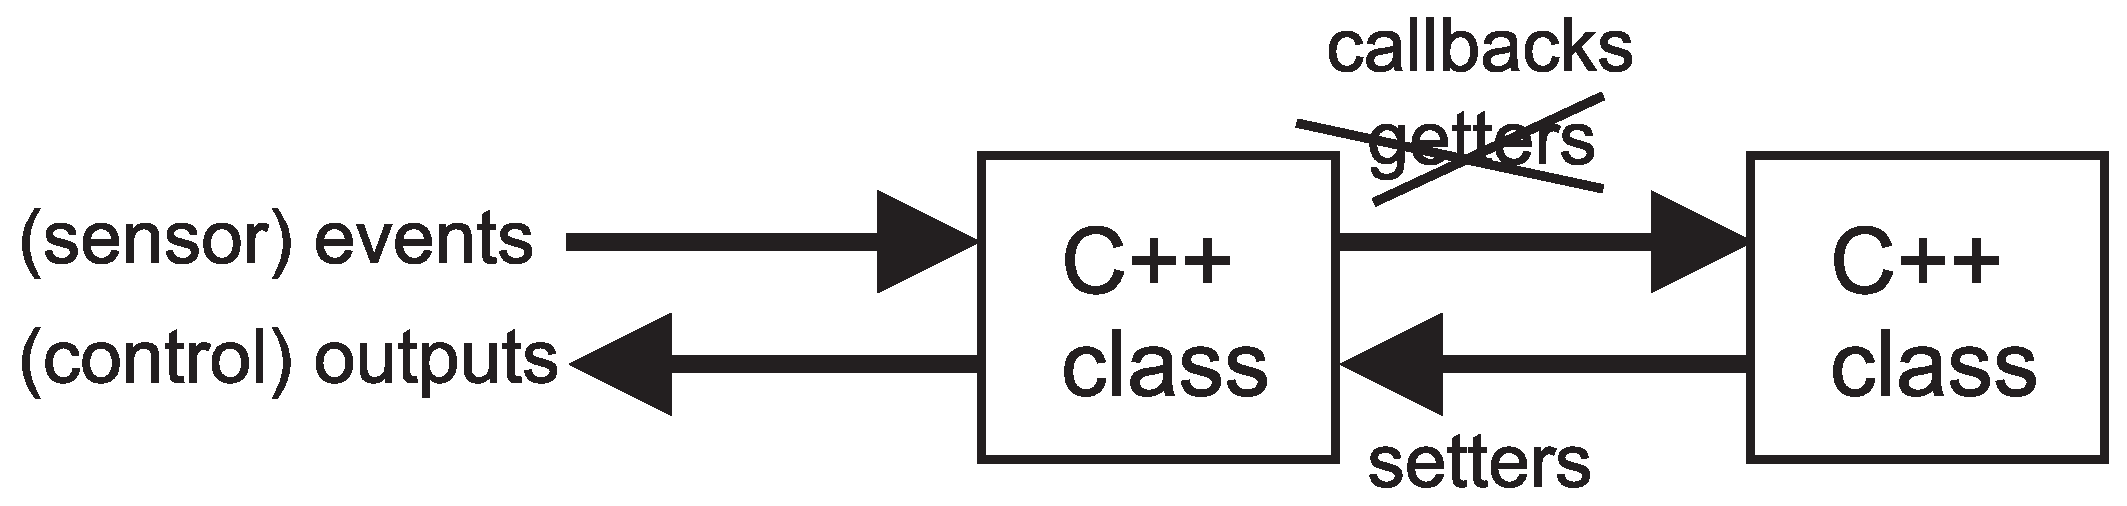
\includegraphics[width=\textwidth]{gettersetters}}
    \end{center}
    A realtime system with two C++ classes. Communication
      between classes is achieved with callbacks (not getters) for incoming events
      and setters to send out control events. The control output itself
      receives its timing from the events so that the loop is traversed
      as quickly as possible.
    \end{figure}
\end{frame}


\begin{frame}[fragile]
    \frametitle{C++ callback interface}

Callback interface:
\begin{verbatim}
class LSM9DS1callback {
public:
        virtual void hasSample(LSM9DS1Sample sample) = 0;
};
\end{verbatim}

C++ driver class:
\begin{verbatim}
void LSM9DS1::dataReady() {
        LSM9DS1Sample sample;
        // fills the sample struct with data
        // ...
        lsm9ds1Callback->hasSample(sample);
}
\end{verbatim}

C++ driver callback registration:
\begin{verbatim}
void LSM9DS1::registerCallback(LSM9DS1callback* cb);
\end{verbatim}

\end{frame}



\begin{frame}[fragile]
    \frametitle{Merging C++ driver class and callback interface}
Instead of creating a separate class containing the callback you
can also add the callback straight to the device driver class.
\begin{verbatim}
class ADS1115rpi {
        ...
        virtual void hasSample(float sample) = 0;
        ...
};
\end{verbatim}
This forces the client to implement the callback to be able to use
the class. This creates a very safe environment as all dependencies
are set at compile time and the abstract nature of the base class
makes clear what needs to be implemented.
See
\url{https://github.com/berndporr/rpi_ads1115} for a complete example.
\end{frame}



\begin{frame}[fragile]
    \frametitle{Event timing: GPIO events}

    \begin{verbatim}
class mySensorClass {
    static void gpioISR(int g, int l, uint32_t, void* usr)
    ...
}
        \end{verbatim}
        is registered with pigpio:
        \begin{verbatim}
gpioSetISRFuncEx(24,RISING_EDGE,ISR_TIMEOUT,gpioISR,
                 (void*)this);
        \end{verbatim}
        The callback registered will then be \texttt{this->dataReady()}.
        \begin{verbatim}
class LSM9DS1 {
    void dataReady();
    static void gpioISR(int gpio, int level, uint32_t tick, void* userdata)
    {
        ((LSM9DS1*)userdata)->dataReady();
    }
};
        \end{verbatim}

\end{frame}




\begin{frame}[fragile]
\frametitle{Event timing: blocking I/O}
Thread workers with endless loops are often used in conjunction with blocking
I/O which provide the timing:
\begin{verbatim}
void run() {
       running = true;
       while (running) {
              read(buffer); // blocking
              doCallback(buffer); // hand data to client
       }
}
\end{verbatim}
\end{frame}



\begin{frame}[fragile]
  \frametitle{Event timing: \texttt{select()}}
Non-blocking I/O and \texttt{select()}
which waits till data has become available.
\begin{verbatim}
FD_ZERO(&rdset);
FD_SET(fileno,&rdset);
struct timeval timeout;
timeout.tv_sec = 0;
timeout.tv_usec = 500000;
int ret = select(fileno+1,&rdset,NULL,NULL,&timeout);
if (ret < 0) return ret;
// non-blocking I/O read
ret = read(fileno,buffer,bytes_per_sample * n_chan);
\end{verbatim}
\end{frame}



\begin{frame}[fragile]
  \frametitle{Event timing: \texttt{poll()}}
  \texttt{poll()} is similar to \texttt{select()} but
  has less temporal resolution (ms) to wake up a thread.
  Here used to wake up a thread after a GPIO pin has been
  triggered in \texttt{/sys}:
\begin{verbatim}
int SysGPIO::gpio_poll(int gpio_fd, int timeout) const
{
  struct pollfd fdset[1] = {};
  int nfds = 1;
  char buf[MAX_BUF] = { 0 };
  fdset[0].fd = gpio_fd;
  fdset[0].events = POLLPRI;

  int rc = poll(fdset, nfds, timeout);

  if (fdset[0].revents & POLLPRI) {
    (void)read(fdset[0].fd, buf, MAX_BUF);
  }
  return rc;
}
\end{verbatim}
\end{frame}


\begin{frame}[fragile]
\frametitle{Timing with Linux/pigpio timers}
As a \textsl{last resort} one can use a timer. Similar to threads one can
create timers which are then called at certain intervals. As with threads
timers should be \textsl{hidden} within a C++ class as
\textsl{private} members which then trigger \textsl{public callbacks}
via C++ callback mechanisms as described above.

Generally it's \textsl{not recommended}
to use timers for anything which needs to be reliably sampled, for
example ADC converters or sensors with sampling rates higher than a
few Hz. On the raspberry PI use the pigpio library and its timer
callbacks --- if needed at all.
\end{frame}


\begin{frame}[fragile]
  \frametitle{How does an event driven main() look like?}
 \begin{verbatim}
int main() {
   Camera camera;
   AI ai;
   GUI gui;
 
   gui.register(&ai);
   ai.register(&camera);

   camera.start();
   ai.start();

   gui.exec(); // blocking till user shuts it down

   ai.stop();
   camera.stop();
   return 0;
} 
\end{verbatim}
\end{frame}

\end{document}
